\subsection{Klassifizierung von Audiodateien durch ein Neuronales Netz}
Durch das neuronale Netz sollen digitale Audiodateien (Audiosamples) mit variabler Länge in fünf Merkmalsklassen klassifiziert werden. Dabei kann ein Datenpunkt, also ein Audiosample, mehreren Merkmalsklassen zugehörig sein. Dies wird als ``Multi-Label-Klassifizierung`` bezeichnet \cite{multilabel-classification}. Wird eine Audiodatei (Eingabevektor) zur Klassifizierung in das neuronale Netz eingegeben, erhält man als Ausgabe einen Ausgabevektor von fünf Werten zwischen 0.00 und 1.00, wobei jeder der fünf Werte  die Ähnlichkeit mit einer der fünf Merkmalsklassen repräsentiert (0.00 $\equiv$ keine Ähnlichkeit, 1.00 $\equiv$ Übereinstimmung). Die Merkmalsklassen werden wie folgt definiert:
\begin{itemize}
	\item \textbf{bass:} Das Audiosample enthält Töne aus dem tiefen Frequenzspektrum
	\item \textbf{pitched:} Das Audiosample enthält Töne aus dem hohen Frequenzspektrum
	\item \textbf{melodic:} Das Audiosample enthält melodische Elemente
	\item \textbf{rhythmic:} Das Audiosample enthält rhytmische Elemente
	\item \textbf{sustained:} Das Audiosample enthält ``flächige`` Elemente, also ``langgezogene`` Töne
\end{itemize}

Dieses neuronale Netz wird mit selbst generierten Trainingsdaten trainiert und anschließend als fertiges Modell mittels dem STM32 proprietären Tool ``STM32Cube.AI`` in C-Code umgewandelt. Damit kann das Neuronale Netz im eigenen Code als normale C-Funktion verwendet werden, mit dem Eingabevektor (Audiodaten) als Funktionsparameter und dem Ausgabevektor (Klassifikationsergebnis) als Rückgabewert. \cite{stm32-cube-ai-documentation}

\begin{wrapfigure}{r}{0.4\textwidth}
	\centering
	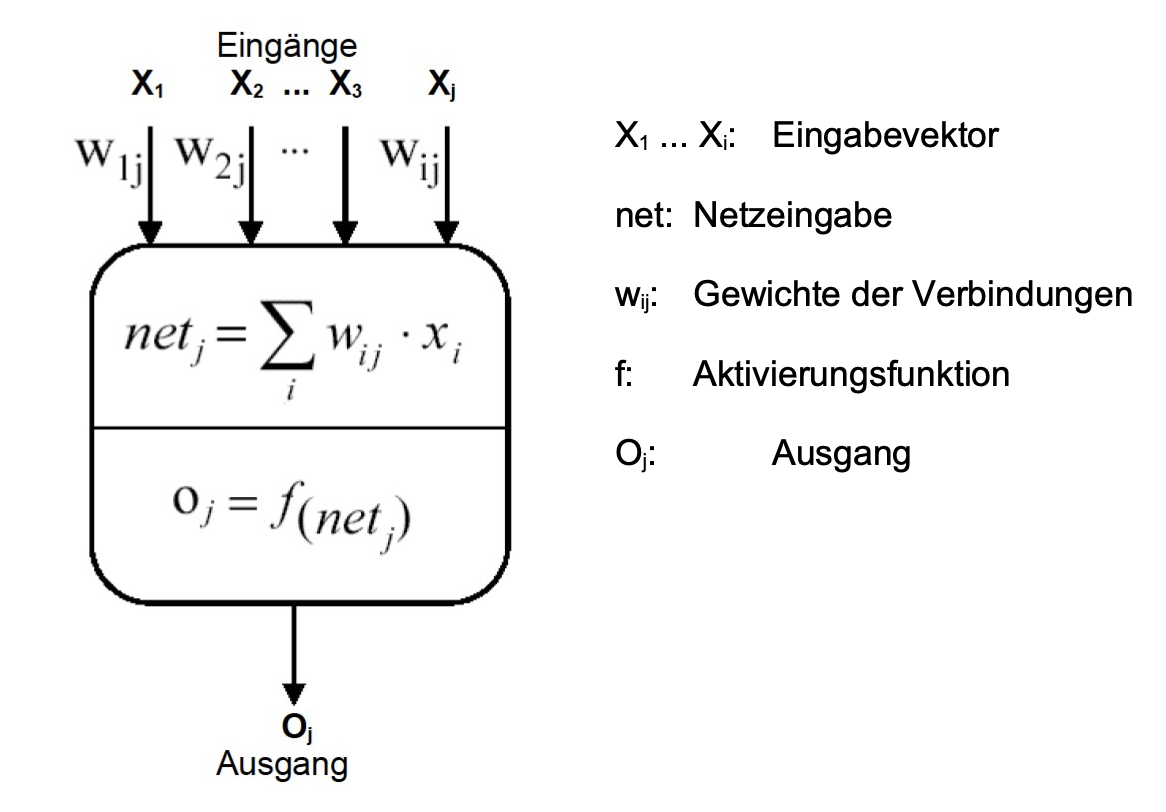
\includegraphics[width=0.4\textwidth]{images/08_durchfuehrung/neuron-aufbau.png}
	\caption{Aufbau des künstlichen Neurons. Quelle: Thieling, Lothar: “Neuronale Netze (Vorlesungsskript ML)”, Kapitel F, Seite 6.}
	\label{fig:img-aufbau-neuron}
\end{wrapfigure}

Die Umwandlung in C-Code ist mögich, da ein künstliches Neuron, wie in \textbf{\autoref{fig:img-aufbau-neuron}} dargestellt, aus aus mehreren Gewichten (\textit{W\textsubscript{x}}) in Form eines Vektors besteht, der mit dem Eingabevektor (\textit{X\textsubscript{n}}) des Neurons multipliziert wird. Beide Vektoren sind Fließkommazahlen. Anschließend werden diese Produkte aufaddiert und als Eingabewert einer mathematischen Funktion, der sog. ``Aktivierungsfunktion`` (\textit{f}) verwendet. Der Ausgabewert dieser Funktion ist die Ausgabe des Neurons. \cite{neural-network-basics}

Bei einem neuronalen Netz werden die Neuronen in Schichten hinterheinander angeordnet, die Neuronen der benachbarten Schichten werden vereinfacht gesagt miteinander verbunden, also die Eingabe des einen Neurons bildet eine der Eingaben des nachfolgenden Neurons. \cite{neural-network-basics}

Sowohl die Multiplikation von Vektoren, als auch die Berechnung von Funktionswerten ist in der Programmiersprache C problemlos möglich.

Der ressourcenintensive Teil des Umgangs mit neuronalen Netzen ist das Training, also der Anpassung der Gewichtswerte bis das Neuronale Netz akzeptable Ausgabewerte liefert \cite{neural-network-basics}. Bei diesem Prozess müssen vergleichsweise sehr viele Berechnungen durchgeführt werden. Aus diesem Grund wird das Neuronale Netz zuerst trainiert und erst dann als fertiges Modell in C-Code ungewandelt und auf dem STM32 Microcontroller betrieben. 
Dass das Neuronale Netz fortlaufend durch Benutzerinteraktion weiter trainiert wird, ist nicht vorgesehen.


\subsubsection{Ansatz für die Klassizierung von Audiodaten}
\label{sec:approach-audio-classification}
Die Audiosamples liegen als WAVE-Dateien (Dateiendung .wav) vor. Diese enthalten in der Regel pulsweitenmodulierte (PCM) Audiodaten \cite{wav-contains-pcm-data}. Da die Daten nicht komprimiert sind, gehören sie in der Audio- und Musikindustrie zu den gängigsten Dateiformaten \cite{wav-popular-file-format-music-industry}. Eine typische Samplerate für WAVE-Dateien beträgt 44,1 kHz, also 44.100 Samples pro Sekunde, wobei ein Sample in der WAVE-Datei ein quantisierter Amplitudenwert zu einem bestimmten Zeitpunkt ist \cite{wav-pcm-data}. Plottet man dies als Graph, könnte ein Audiosignal wie in \textbf{\autoref{fig:img-pcm-graph}} aussehen.


\begin{figure}[h!]
	\centering
	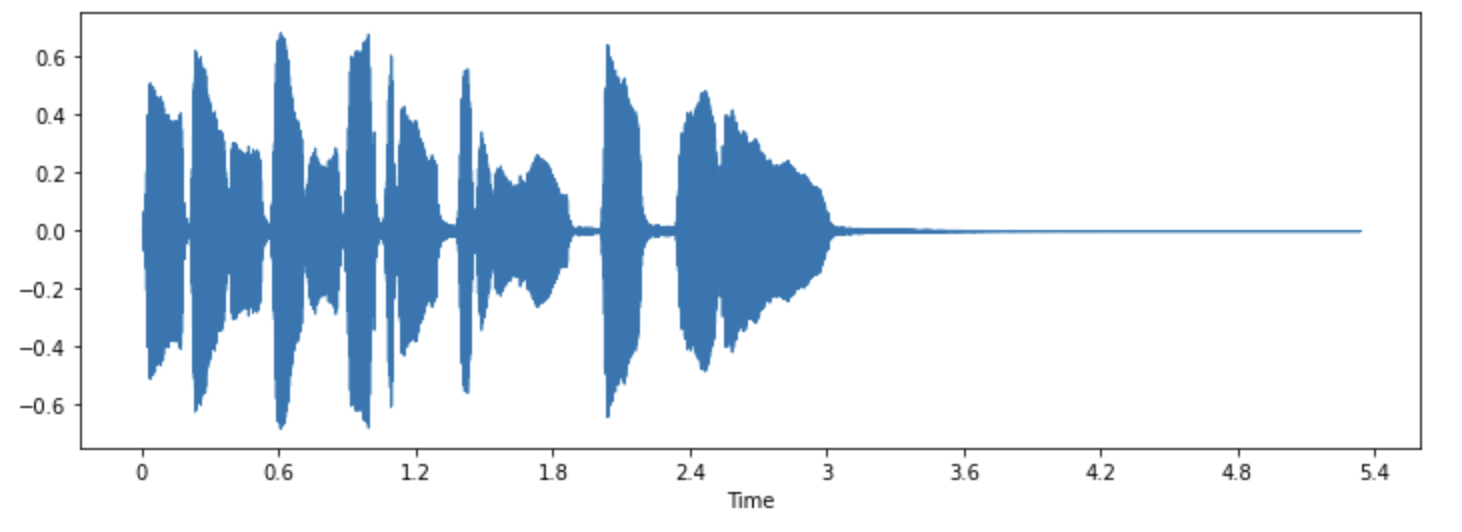
\includegraphics[width=0.6\textwidth]{images/08_durchfuehrung/waveform_plot.png}
	\caption{Darstellung eines PCM Audiosignals, Quelle:  https://huggingface.co/learn/audio-course/chapter1/audio\_data TODO }
	\label{fig:img-pcm-graph}
\end{figure}

Diese Daten direkt durch ein neuronales Netz klassifizieren zu lassen, ist aus verschiedenen Gründen wenig praktikabel. Die zwei Hauptgründe sind die Merkmalsextraktion und die Größe des Eingabevektors. Letzterer Punkt würde dazu führen, dass selbst bei einer geringeren Samplerate von 16 kHz der Eingabevektor 16.000 Werte umfasst. Ein Downsampling auf eine deutlich geringere Zahl, z.B. 1000, ist aufgrund des Shannon-Nyquist-Theorems nicht praktikabel, da dieses besagt, dass die Samplerate mindestens doppelt so hoch sein muss wie die höchste Frequenz \cite{nyquist}. Damit läge der klassifizierbare Frequenzbereich nur im Bereich von \textit{0 Hz} bis maximal \textit{1000 / 2 = 500 Hz}.

Deutlich geeigneter ist es, die Daten als Spektrogramm (Amplitude der verschiedenen Frequenzen eines Signals über die Zeit) wie in \textbf{\autoref{fig:img-spectrogram}} darzustellen und mit einem Convolutional Neural Network (CNN) zu klassifizieren. CNNs werden in erster Linie zur Klassifizierung von Bildern eingesetzt. Die wesentliche Idee ist, dass das neuronale Netz dann nicht nur klassifiziert, sondern auch die Bildvorverarbeitung und die Merkmalsextraktion übernimmt \cite{how-cnn-work}. Da die Audiodateien für das menschliche Gehör klassifiziert werden, sind Mel-Spektrogramme besonders geeignet. Sie basieren auf der Mel-Skala, die das menschliche Gehör nachahmt. Die Mel-Skala ist eine nichtlineare Skala der Frequenzen, die mehr Gewicht auf tiefere Frequenzen legt \cite{mel-spectrogram}.

\begin{figure}[h!]
	\centering
	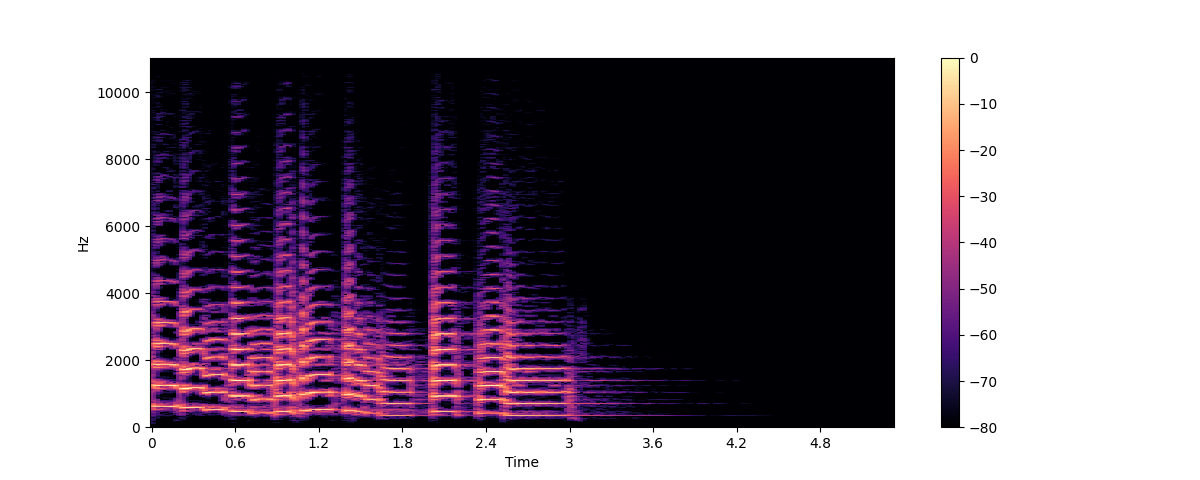
\includegraphics[width=0.75\textwidth]{images/08_durchfuehrung/spectrogram_plot.png}
	\caption{Darstellung eines Audiosignals als Spektrogramm, Quelle:  https://huggingface.co/learn/audio-course/chapter1/audio\_data TODO }
	\label{fig:img-spectrogram}
\end{figure}

Der limitierende Faktor beim Einsatz eines CNN auf einem Microcontroller sind die Hardwareressourcen, also in erster Linie Flash-Speicher und RAM.

Aufgrund der fehlenden Erfahrungswerte der Teammitglieder mit der möglichen Komplexität von neuronalen Netzen, die mit den Hardwareressourcen eines Microcontrollers betrieben werden können, wird sich auf ein Beispielprojekt von STMicroelectornics gestützt. Dieses heißt ``Acoustic Scene Classification`` \cite{stm-asc}\cite{stm-asc-2}. Kern ist die Klassifizierung von 30x32 px großen Mel-Spektrogrammen mit einem zwei Schichten CNN, die einen Eingabevektor von \textit{32 x 30 = 960} Werten ergeben. 

Sowohl die Dimensionierung der Spektrogramme, als auch die Topologie des Neuronalen Netzes, die Anzahl der Neuronen je Schicht und Elemente der Datenvorverarbeitung wurden aus diesem Projekt übernommen. Damit ist sicher gestellt, dass das Neuronale Netz am Ende nicht die Ressourcen des Microcontrollers übersteigt.

\subsubsection{Generieren der Eingabedaten}
\label{sec:input-data-generation}
Für das Training des neuronalen Netzes sind Trainingsdaten erforderlich. Diese bestehen aus Eingabedaten, die bereits mit den korrekten Klassifikationsergebnissen, also Labels, versehen sind. Um das Training des neuronalen Netzes während des Trainings einschätzen und nach Abschluss des Trainings validieren zu können, werden die Eingabedaten in drei Segmente aufgeteilt.

Da online keine kostenlosen und bereits mit den passenden Labels versehene Datensätze gefunden werden konnten, wurden eigene Daten generiert. Grundlage hierfür bildet eine private Audiosample-Bibliothek. Ein eigens entwickeltes Python-Skript ermöglicht es, Audiosamples auszuwählen, abzuspielen und zeiteffizient zu labeln.

Für jedes manuell gelabelte Audiosample wird eine eindeutige Identifikationsnummer (UID) generiert. Die zugehörigen Labels werden in einer CSV-Datei gespeichert. Ein Beispiel für einen solchen Datensatz zeigt \textbf{\autoref{tab:audiodaten}}. Außerdem wird eine Kopie des Audiosamples unter dem Namen der UID im Ausgabeordner des Skripts abgelegt. Diese Dateien werden später vom Jupyter-Notebook für das Training verwendet.

\begin{table}[h!]
	\centering
	\begin{tabular}{|m{2.8cm}|m{4.5cm}|m{0.8cm}|m{1.2cm}|m{1.5cm}|m{1.5cm}|m{1.3cm}|}
		\hline
		\textbf{UID} & \textbf{File} & \textbf{bass} & \textbf{pitched} & \textbf{sustained} & \textbf{rhythmic} & \textbf{melodic} \\ \hline
		ecfad96b740844c3
		9c96127279f22cf6 &  BD 606 Long MPC60 01.wav & 1 & 0 & 0 & 1 & 0 \\ \hline
	\end{tabular}
	\caption{Beispielhafter Datensatz eines Audiosamples}
	\label{tab:audiodaten}
\end{table}

Bei der Auswahl der Audiosamples wurde darauf geachtet, dass die Daten annähernd gleich verteilt sind, um eine ausgewogene Trainingsbasis zu schaffen. Ein Ungleichgewicht in den Daten kann sich negativ auf das Training und die Klassifikationsergebnisse auswirken. Überrepräsentierte Merkmale könnten die Klassifikationsschwellenwerte beeinflussen, sodass die häufiger vorkommenden Klassen später bevorzugt erkannt werden. Wie in \textbf{\autoref{tab:img-class-spread-graph}} zu sehen, ist die Gleichverteilung jedoch zugegebenermaßen nur mäßig gelungen und hätte einen größeren Zeitaufwand erfordert.

\begin{figure}[h!]
	\centering
	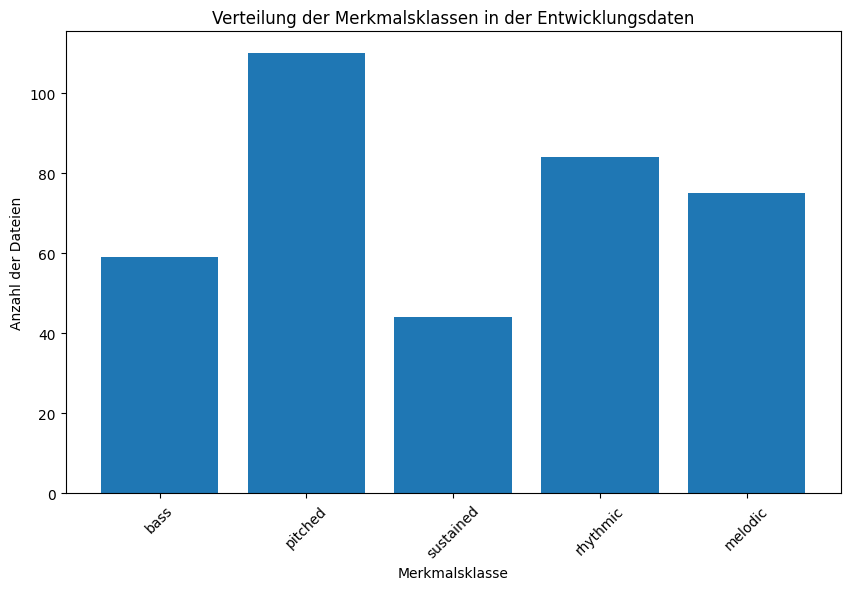
\includegraphics[width=0.75\textwidth]{images/08_durchfuehrung/class_spread_plot.png}
	\caption{Repräsentation der verschiedenen Merkmalsklassen in den Entwicklungsdaten}
	\label{fig:img-class-spread-graph}
\end{figure}

Zudem wurde sichergestellt, dass der Variationsbereich jeder Klasse möglichst umfassend abgedeckt ist. Dies umfasst sowohl reine Formen jeder Klasse – beispielsweise bei „pitched“ Audiosamples ausschließlich mit Tönen aus dem hohen Frequenzbereich – als auch Mischformen, die Merkmale mehrerer Klassen kombinieren.

Insgesamt wurden 207 Audiosamples unterschiedlicher Länge mit Labels versehen.

Insgesamt wu
TODO:

- wie viele Eingabe-Audiosamples

- wie viele Trainingsdatensätze

- Aufteilung der Daten (Grafik)

- Quellen

\subsubsection{Datenvorverarbeitung}

Für die Datenvorverarbeitung und das Training des neuronalen Netzes wird ein Jupyter-Notebook verwendet. Dieses ermöglicht eine Kombination aus formatiertem Text und Python-Code, was die Lesbarkeit und Nachvollziehbarkeit des Codes erleichtert.

Damit die gelabelten Daten für das Training des neuronalen Netzes verwendet werden können, müssen sie zunächst aufbereitet bzw. vorverarbeitet werden. Um die zu verarbeitenden Datenmengen sinnvoll zu verringern, wird zunächst die Samplerate aller Audiosamples auf 16 kHz reduziert.

Wie im Abschnitt \ref{sec:input-data-generation} erwähnt, liegen die Audiosamples als WAVE-Dateien unterschiedlicher Längen vor. Die in Abschnitt \ref{sec:approach-audio-classification} beschriebenen Dimensionen der durch das neuronale Netz klassifizierbaren Mel-Spektrogramme betragen 32x30 Pixel. Um bei unterschiedlich langen Audiosamples die zeitliche Abhängigkeit zu bewahren und auch bei längeren Audiosamples wichtige Informationen im Spektrogramm abzubilden, müssen die Audiosamples in Sektionen gleicher Länge unterteilt werden, wobei später aus jeder Sektion ein Spektrogramm erstellt wird. Diese Sektionen werden im Folgenden als „Audiosubsamples“ bezeichnet.

Ein Audiosubsample, also ein Mel-Spektrogramm, entspricht dabei 16.384 Frames, was bei einer Samplerate von 16 kHz etwas mehr als einer Sekunde entspricht. Analog zum Beispielprojekt „Acoustic Scene Classification“ \cite{stm-asc}\cite{stm-asc-2} werden die Audiosubsamples anschließend mittels eines „Sliding Window“ in 1024 Samples lange, um 512 Samples überlappende, Frames unterteilt. Diese Überlappung stellt sicher, dass Informationen zu den Anfangs- und Endzeitpunkten der Frames nicht durch das „Abschneiden“ verloren gehen. Die Aufteilung der Audiosamples in Audiosubsamples und Frames wird in \textbf{\autoref{fig:img-audiosubsamples-frames-overview} }visualisiert.

\begin{figure}[h!]
	\centering
	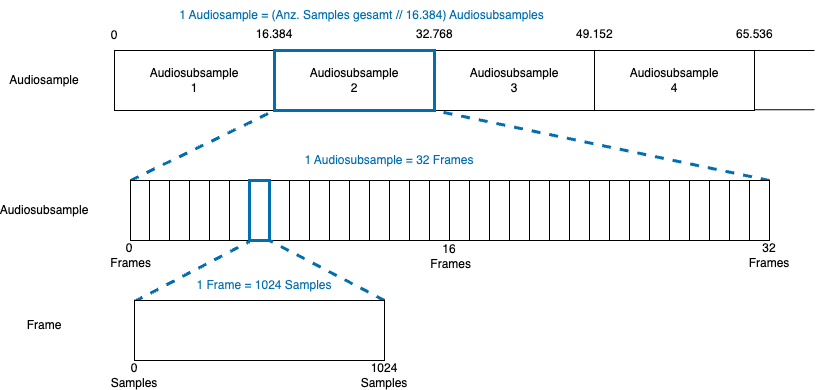
\includegraphics[width=0.8\textwidth]{images/08_durchfuehrung/audiosubsamples_frames_overview.png}
	\caption{Darstellung der Unterteilung der Audiosamples in Audiosubsamples und Frames}
	\label{fig:img-audiosubsamples-frames-overview}
\end{figure}

Das Sliding Window Prinzip, mit dem Audiosubsamples in überlappende Frames unterteilt werden, ist in \textbf{\autoref{fig:img-sliding-window}} dargestellt.

\begin{figure}[h!]
	\centering
	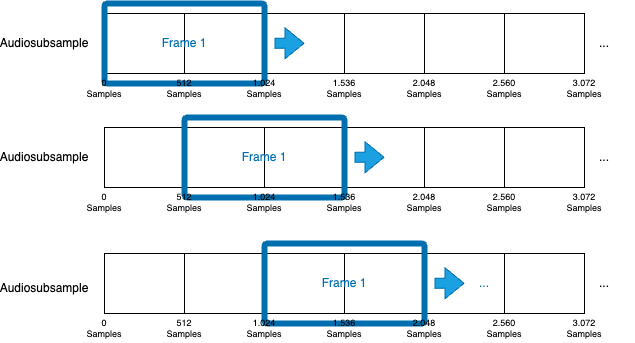
\includegraphics[width=0.7\textwidth]{images/08_durchfuehrung/sliding_window.png}
	\caption{Darstellung des Sliding Window Prinzips}
	\label{fig:img-sliding-window}
\end{figure}

Nun können die Mel-Spektrogramme erstellt werden. Eine Spalte des Spektrogramms wird dabei aus einem Frame berechnet. Setzt man die 32 in einem Audiosubsample enthaltenen Frames, also Spektrogramm-Spalten, zusammen, erhält man das 32x30 Pixel große Spektrogramm für ein Subsample.

Abschließend müssen die erhaltenen Daten standardisiert, also mittelwertfrei gemacht werden. Dies ist beim maschinellen Lernen üblich und sorgt dafür, dass das Modell schneller und effizienter konvergiert, indem es die Varianz in den Eingabedaten reduziert und eine gleichmäßige Verteilung der Werte gewährleistet. Damit diese Standardisierung später beim Einsatz des neuronalen Netzes auf dem Mikrocontroller nachgeahmt werden kann, werden die Werte des Scalers, der die standardisierten Werte berechnet, exportiert.


\subsubsection{Aufteilen der Eingabedaten in Trainings- Test und Validierungsdaten}

\subsubsection{Training des Neuronalen Netzes}

TODO:

- Topologie

- Trainignsparameter und warum (Adam (?), Learning Rate, no. epochs, etc.)

- erklären wann Training zu Ende

- accuracy bla graph

- confusion matrix

- model.h5

(und in Validierng einfach nur eigene samples eingeben und schauen bzw. hier drauf verweisen)




\subsubsection{Betrieb des Neuronalen Netzes auf dem STM32 Microcontroller}
TODO:

- wieder Datenvorverarbeitung

- Scaler

- Vorgehen Cube.AI (model.h5)

- Inference Zeit

- Verweis auf Validierungs-Kapitel